\documentclass[a4paper,12pt,landscape]{article}
% border: 边距
\usepackage{amsmath}
\usepackage{amsthm}
\usepackage{amssymb}
\usepackage{mathtools}
\usepackage{amsfonts}
\usepackage{stmaryrd} %% \llbracket \rrbracket

\usepackage{graphicx}
\usepackage{color}
\usepackage{geometry}
\geometry{left=2cm,right=2cm,top=1.5cm,bottom=1.5cm}

\usepackage{tikz}\usetikzlibrary{backgrounds}
%%=============================================================================
\begin{document}


\begin{itemize}
    \item 
    For deterministic classes, $\mathcal{C} = $ co-$\mathcal{C}$.

    \item $\mathrm{P}$ is considered the only \textit{tractable} complexity class.

    \item \textbf{Satisfiability} and \textbf{validity} are complementary problems, 
    hence determining that satisfiability is in $\mathcal{C}$ immediately implies that validity is in co-$\mathcal{C}$,  
    and vice versa.

    \item 
\end{itemize}


\[
    sdfasdfqweasdfs
\]


\[\begin{array}{ccccccccccccc}
    \mathrm{P} & \subseteq & \mathrm{NP} & \subseteqq & \mathrm{PSPACE} & \subseteq & \mathrm{EXPTIME} & \subseteq & \mathrm{NEXPTIME} & \subseteq \\   

    &  \subseteq & \mathrm{EXPSPACE} & \subseteq & \mathrm{2EXPTIME} & \subseteq & \mathrm{N2EXPTIME} & \cdots & \mathrm{ELEM} \\
\end{array}\]



% figure
\begin{figure}[ht!]
    \centering
    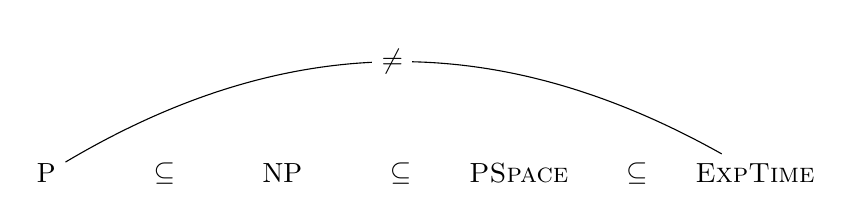
\begin{tikzpicture}[node distance=1.5cm]
        \node (p) at (0,0) {$\mathrm{P}$};
        \node (s1) [right of=p] {$\subseteq$};
        \node (np) [right of=s1] {$\mathrm{NP}$};
        \node (s2) [right of=np] {$\subseteq$};
        \node (pspace) [right of=s2] {\textsc{PSpace}};
        \node (s3) [right of=pspace] {$\subseteq$};
        \node (exptime) [right of=s3] {\textsc{ExpTime}};

        
        \draw (p) to [bend left]node[fill=white]{$\not=$} (exptime);

    \end{tikzpicture}
\end{figure}


\vspace{1.5em}








\begin{table}[ht!]
    \begin{center}
    \renewcommand{\arraystretch}{1.3} % 行距
    \renewcommand{\arraycolsep}{1.2em} % 列距
    \begin{tabular}{c|lllr}
    \hline
    P & 
    \\
    
    
    \rotatebox[origin=c]{270}{$\subseteq$} \\

    
    NP & 
    $PL_{Sat} = \mathbf{S5}_{Sat}$: NP-complete &
    & 
    $PL_{Valid}$: co-NP-complete\\

    
    \rotatebox[origin=c]{270}{$\subseteq$} \\

    
    \textsc{PSpace} & 
    $\mathbf{K}_{Sat} = \mathbf{T}_{Sat} = \mathbf{S4}_{Sat} =  QBF_{Sat}$ = $QBF_{Valid}$: \textsc{PSpace}-complete\\

    
    \rotatebox[origin=c]{270}{$\subseteq$} \\

    
    \textsc{ExpTime} & 
    $PDL_{Sat}$ = $PDL_{Valdi}$: \textsc{ExpTime}-complete \\


    \hline
\end{tabular}
\end{center}

\vspace{1.5em}

$PL$: propositional logic. \\
$QBF$: the logic of quantified Boolean formulas. \\
$PDL$: propositional dynamic logic. \\
\end{table}



PSPACE and EXPTIME are deterministic complexity classes, co-PSPACE is identical to PSPACE and co-EXPTIME is identical to EXPTIME





\vspace{1.5em}




\begin{table}[htp!]
    \caption{The complexity of the satisfiability problem for modal logics.}
    \label{tab: complexity-of-modal-logic}
    \vspace{.3em}
    \begin{center}
    \renewcommand{\arraystretch}{1.7} % 行距
    \renewcommand{\arraycolsep}{1.5em} % 列距
    \begin{tabular}{llllll}
    \hline
    \multicolumn{1}{c}{NP-complete} & 
    \multicolumn{1}{c}{PSPACE-complete} &  
    \multicolumn{1}{c}{EXPTIME-complete} &  
    \multicolumn{1}{c}{NEXPTIME-complete} & 
    \multicolumn{1}{c}{undicidable} \\
    \hline

    $\mathbf{PL}$, $\mathbf{S5}, \mathbf{KD45}$ 
    & 
    $\mathbf{K}_n, \mathbf{T}_n, \mathbf{S4}_n$, $n \geq 1$
    & 
    $\mathbf{K}^C_n, \mathbf{T}^C_n$, $n \geq 1$
    \\


    & 
    $\mathbf{S5}_n, \mathbf{KD45}_n$, $n \geq 2$ 
    &
    $\mathbf{S4}^C_n,\mathbf{S5}^C_n, \mathbf{KD45}^C_n$, $n \geq 2$ 
    \\


    $\mathrm{NEXT}(\mathbf{S4.3})$
    & 
    $\mathbf{QBF}$ 
    &   
    $\mathbf{PDL}$ \\

    &
    &
    $\mathbf{K}^{\mathsf{E,A}}$ \\

    &
    &
    &
    $\mathbf{S5} \times \mathbf{S5}$, $\mathbf{S5} \times \mathbf{K}$   \\ 

    
 

    &&&& 
    $\mathbf{S5}^n$ for $n \geq 3$,  \\
    
    $n \times n$ tiling ($n$ in unary)  &&&
    $n \times n$ tiling ($n$ in binary) &
    $\mathbb{N} \times \mathbb{N}$ tiling  \\
    \hline
\end{tabular}
\end{center}



\begin{itemize}
    \item Cf. [Halpern and Moses, 1992, Table 1, p. 350]
    
    \item In the unary numeral system, $0$ is represented by the empty string $\epsilon$, numbers $1,2,3,\dots$ are represented in unary as $1, 11, 111, \dots$.

    \item $C$: the logic with common knowledge operator
    \item $D$: adding distributed knowledge (intersection operator) to the language does not affect the complexity
    
    \item  in these cases of single-agent for $\mathbf{S4}^C$, $\mathbf{S5}^C$ and $\mathbf{KD45}^C$, 
     common knowledge reduces to knowledge. 

     \item 
     $\mathrm{NEXT}(\mathbf{S4.3})$: any (consistent) normal extension of $\mathbf{S4.3}$. \\
     \textsf{Hemaspaandra's Theorem}: every normal logic extending $\mathbf{S4.3}$ is NP-complete.

     \item 
     $\mathbf{K}^{\mathsf{E,A}}$: 
     the expansion of modal logic $\mathbf{K}$ with the universal modality.
\end{itemize}




\end{table}




\vspace{3em}



$\mathbf{K4}$ is complete w.r.t. the class of all \textit{transitive} Kripke frames, 
and also complete w.r.t. the class of all {\color{purple} \textit{irreflexive, transitive}} Kripke frames. 
That is, 
$\mathbf{K4} = \mathsf{Log}~\mathsf{F}^{tran} = \mathsf{Log}~\mathsf{F}^{irref,tran}$.






%%=============================================================================
\clearpage
\section{Tiling problems}

A \textit{tile} $T$ is a $1 \times 1$ square fixed in orientation with colored edges $right(T), left(T), up(T)$ and $down(T)$ taken from some denumerable set.


A \textit{tiling problem} takes the following form:
\begin{quotation}
    given a finite set $\mathfrak{T}$ of tile types, 
    can we cover a {\color{purple} certain part} of $\mathbb{Z} \times \mathbb{Z}$, 
    using only tiles of this type, 
    in such a way that adjacent tiles have the same color on the common edge.
\end{quotation}



\vspace{1.5em}


There are some titling problems:

\begin{enumerate}
    \item 
    $\mathbb{N} \times \mathbb{N}$ tiling. 

    Given a finite set $\mathfrak{T}$ of tiles, 
    can $\mathfrak{T}$ tile $\mathbb{N} \times \mathbb{N}$?
\end{enumerate}




    The $\mathbb{N} \times \mathbb{N}$ tiling problem is undecidable, 
    it is \textit{re-complete}.






%%=============================================================================
\end{document} 